\documentclass{standalone}

\input{../../fig-config.tex}

% plots
\usepackage{tikz}
\usetikzlibrary{arrows}
\usetikzlibrary{arrows.meta,positioning,calc,3d}
\usetikzlibrary{automata}
\usepackage{tikz-3dplot}
\usepackage{pgfplots}
\pgfplotsset{compat=newest}

\begin{document}
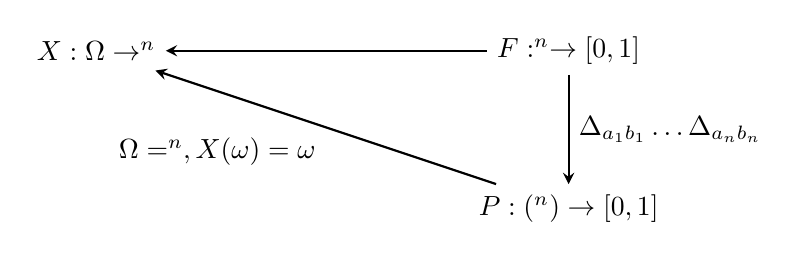
\begin{tikzpicture}[thick]
\node (a) at (0,0) {$X:\Omega\to\R^n$};
\node (b) at (6,0) {$F:\R^n\to[0,1]$};
\draw[-stealth] (b) -- node[above] {} (a);
\node (c) at (6,-2) {$P:\scB(\R^n)\to[0,1]$};
\draw[-stealth] (b) -- node[right] {$\Delta_{a_1b_1}\dots\Delta_{a_nb_n}$} (c);
\draw[-stealth] (c) -- node[below left] {$\Omega=\R^n,X(\omega)=\omega$} (a);
\end{tikzpicture}
\end{document}